\clearpage\section{Thiết kế giao diện và cách đọc kết quả}
Giao diện có bốn khu vực: Trợ lý kiến thức, Thực nghiệm dữ liệu, Bản đồ tri thức và Nguồn \& tài liệu. Mỗi khu vực tương ứng với một nhiệm vụ kiểm tra; khối nhật ký trong cột căn cứ phản ánh lượt đang được chọn. Các hình minh họa ghi lại giao diện và kết quả thực nghiệm trên ứng dụng.

\subsection{Trợ lý kiến thức}
Người dùng nhập câu hỏi hoặc chọn câu hỏi gợi ý. Ví dụ ``HbA1c là gì?'' được gửi đến POST /api/chat với nhiệm vụ kiến thức. Bộ truy xuất tìm tối đa ba đoạn phù hợp; agent đối chiếu phạm vi và agent phản hồi tổng hợp nội dung có mã tài liệu. Người xem cần mở liên kết nguồn và đối chiếu nhật ký, không chỉ đọc câu trả lời. Nếu không có bằng chứng đạt ngưỡng, phản hồi yêu cầu làm rõ. Giao diện khóa nút gửi trong thời gian chờ và hiển thị lỗi kết nối khi yêu cầu thất bại.
\begin{figure}[htbp]\centering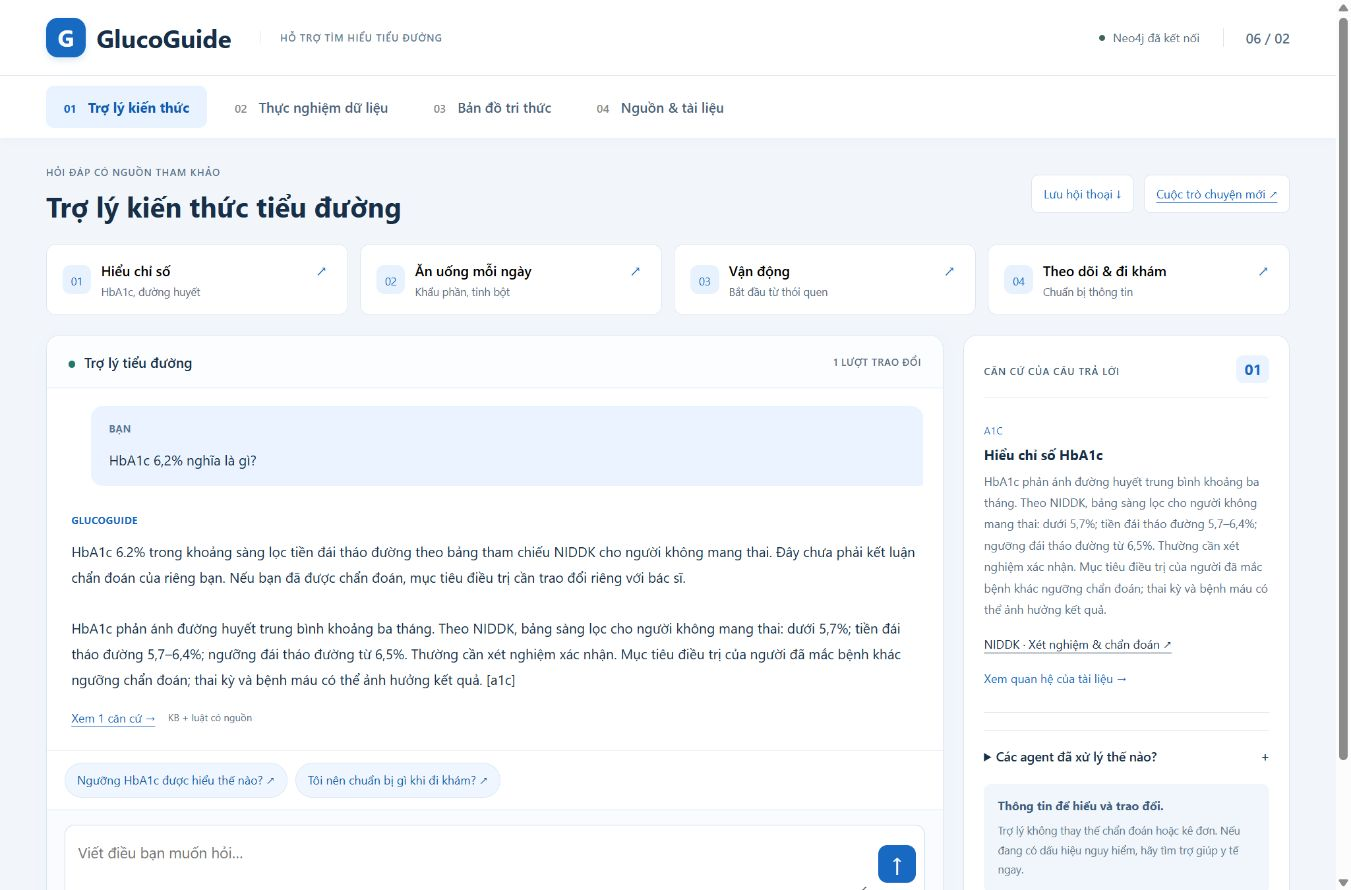
\includegraphics[width=\linewidth,height=.62\textheight,keepaspectratio]{demo-chat.png}\caption{Trợ lý kiến thức: câu trả lời, mã tài liệu và liên kết nguồn.}\end{figure}
\clearpage
\subsection{Thực nghiệm dữ liệu: phân loại}
\productlink{Mở giao diện thực nghiệm}{https://dirt-lucky-capture-mighty.trycloudflare.com/\#models}
Chọn ``Phân loại nhãn tổng hợp'', bấm ``Điền mẫu có sẵn từ dữ liệu'' rồi chạy mô hình MLP. Biểu mẫu gồm tám trường theo đúng schema của checkpoint. API kiểm tra dữ liệu trước khi pipeline điền thiếu, chuẩn hóa và suy luận. Đầu ra là một trong ba nhãn High, Moderate, Low của bộ dữ liệu tổng hợp. Nhãn này không phải xác suất hay chẩn đoán. Kết quả cần đọc cùng macro-F1 và recall lớp Low trong phần thực nghiệm, bởi tập dữ liệu mất cân bằng mạnh.
\begin{figure}[htbp]\centering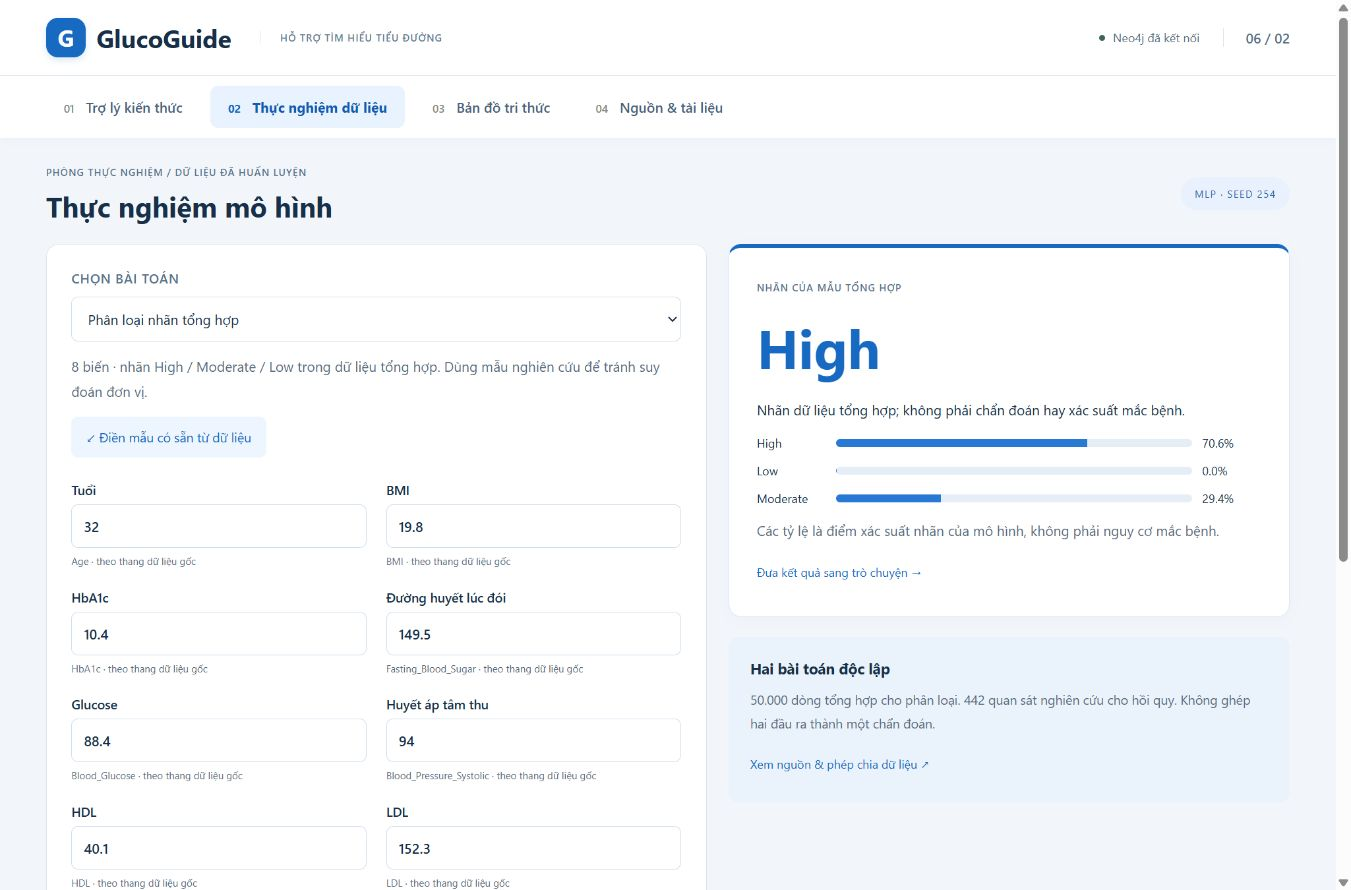
\includegraphics[width=\linewidth,height=.60\textheight,keepaspectratio]{demo-classification.png}\caption{Màn hình phân loại: mẫu đầu vào và nhãn do checkpoint MLP trả về.}\end{figure}
\clearpage
\subsection{Thực nghiệm dữ liệu: hồi quy}
\productlink{Mở giao diện thực nghiệm}{https://dirt-lucky-capture-mighty.trycloudflare.com/\#models}
Chuyển sang ``Dự đoán điểm tiến triển'' để tạo biểu mẫu mười trường. Bấm điền mẫu lại sau khi đổi bài toán; không tái sử dụng tám giá trị của mô hình phân loại. Các tên s1 đến s6 giữ nguyên theo dữ liệu nghiên cứu. Đầu ra là một số thực, được làm tròn hai chữ số trên giao diện; đây là điểm tiến triển sau một năm của bộ diabetes. Bảng kết quả công bố cả Ridge và MLP để thể hiện rằng mô hình sâu không mặc nhiên tốt hơn đối chứng.
\begin{figure}[htbp]\centering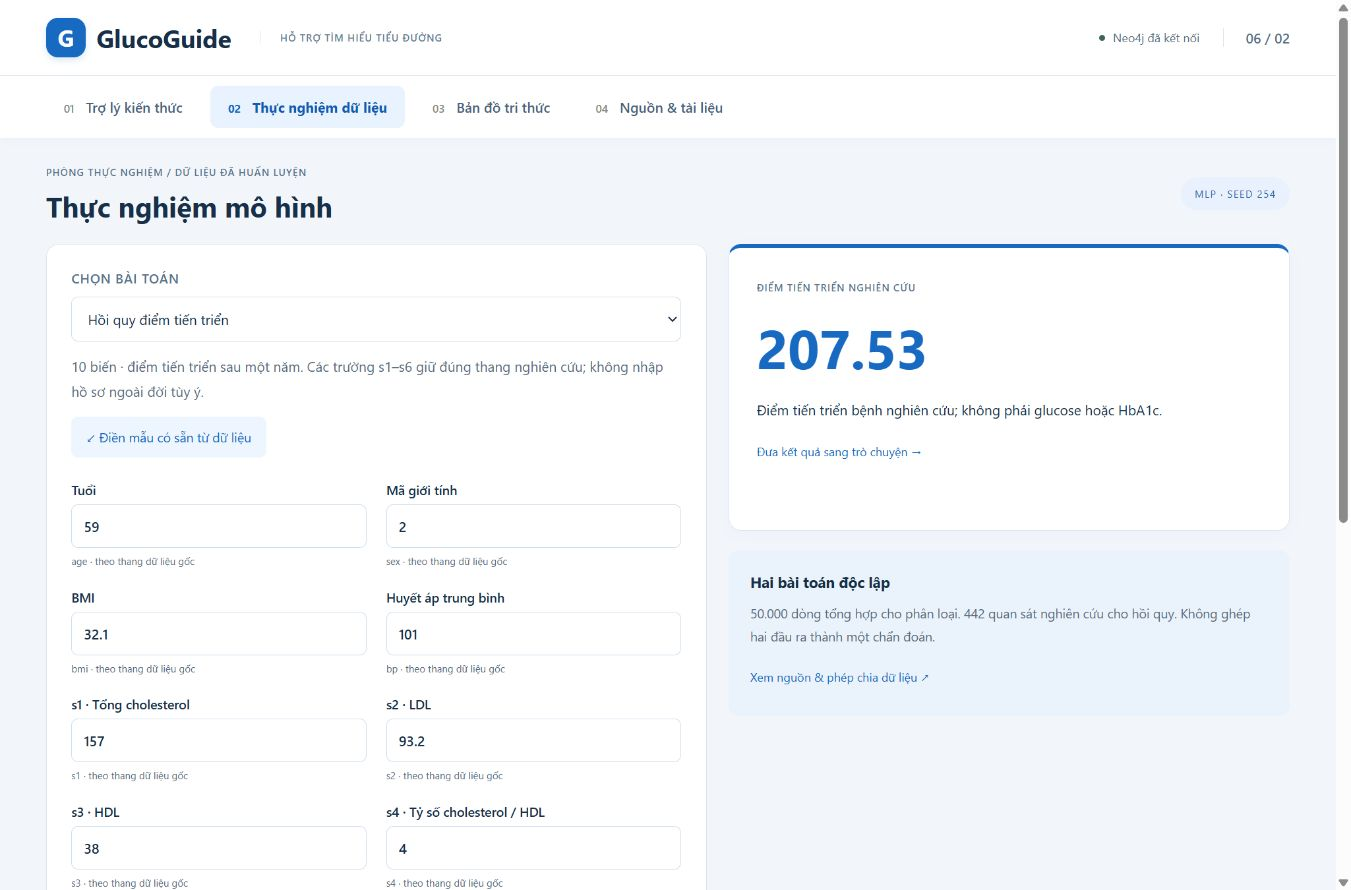
\includegraphics[width=\linewidth,height=.60\textheight,keepaspectratio]{demo-regression.png}\caption{Màn hình hồi quy: biểu mẫu riêng và điểm tiến triển nghiên cứu.}\end{figure}
\clearpage
\subsection{Đồ thị tri thức và đối chiếu Neo4j}
\productlink{Mở giao diện thực nghiệm}{https://dirt-lucky-capture-mighty.trycloudflare.com/\#graph}
Khu vực đồ thị gọi GET /api/graph để đọc các quan hệ thực. Chọn tài liệu a1c để thu nhỏ đồ thị và đọc tên các khái niệm. Bảng cạnh đi kèm thể hiện khái niệm nguồn, quan hệ, khái niệm đích và mã tài liệu. Khi Neo4j không kết nối được, giao diện thông báo lỗi thay vì dựng đồ thị giả. Liên kết Neo4j dùng localhost nên chỉ mở đúng trên máy cài cơ sở dữ liệu; khách xem demo công khai sử dụng đồ thị trong web.
\begin{figure}[htbp]\centering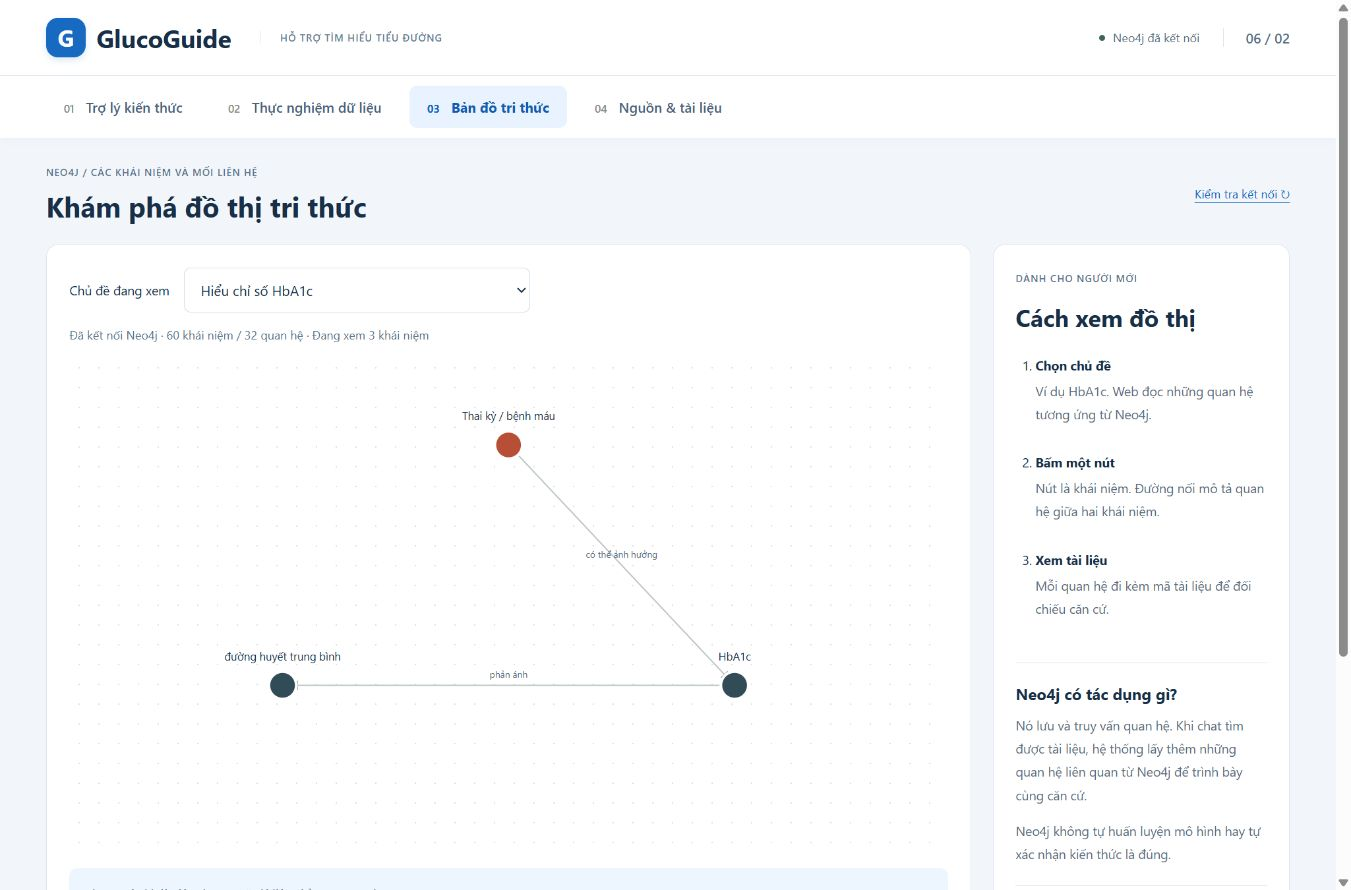
\includegraphics[width=\linewidth,height=.55\textheight,keepaspectratio]{demo-graph.png}\caption{Đồ thị lọc theo tài liệu a1c, lấy từ Neo4j.}\end{figure}
\begin{figure}[htbp]\centering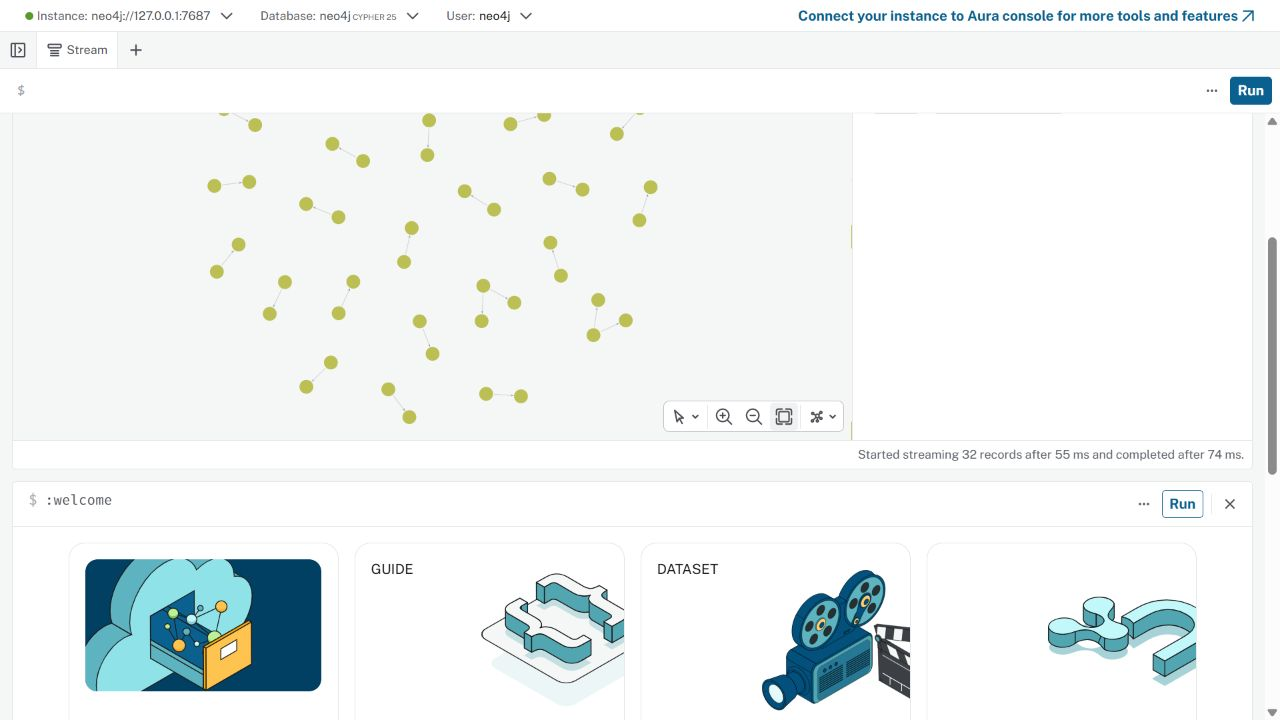
\includegraphics[width=\linewidth,height=.55\textheight,keepaspectratio]{demo-neo4j.png}\caption{Đối chiếu các quan hệ Concept trong Neo4j Browser.}\end{figure}
\clearpage
\subsection{Dữ liệu và nguồn}
\productlink{Mở giao diện thực nghiệm}{https://dirt-lucky-capture-mighty.trycloudflare.com/\#data}
Màn hình thứ tư công bố liên kết bộ dữ liệu, số dòng, số biến, số mẫu train/test và ý nghĩa nhãn. Bảng kiểm kê tám trường phân loại cho biết số giá trị thiếu cùng min, trung vị, max của bản chụp dữ liệu. Danh mục KB liệt kê chín nguồn đang được các đoạn văn sử dụng, kèm mã tài liệu. Bốn mục nguồn chưa được dùng trong registry không được tính vào chín nguồn này.

Nội dung được xuất bởi scripts/audit\_data.py thành web/data\_catalog.json đồng thời với results/data\_audit.json. Khi thay dữ liệu, cần chạy lại bước kiểm kê để đồng bộ báo cáo và web. Kho tri thức hiện là các đoạn văn đã biên soạn; hệ thống chưa có chức năng tải sách hoặc tự thu thập website trong phiên chat.
\begin{figure}[htbp]\centering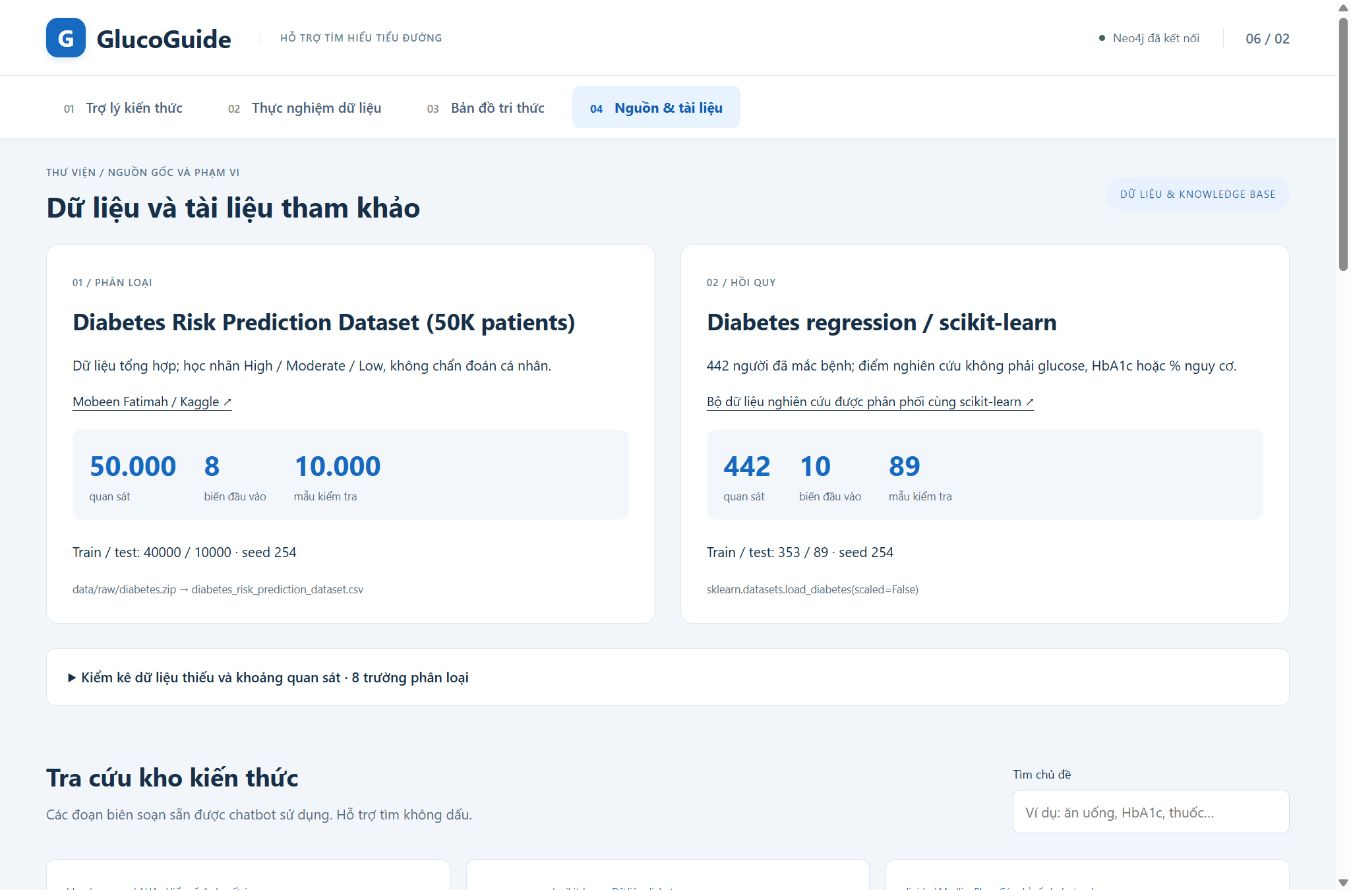
\includegraphics[width=\linewidth,height=.64\textheight,keepaspectratio]{demo-data.png}\caption{Màn hình công bố nguồn gốc và phạm vi hai bộ dữ liệu.}\end{figure}
\clearpage

\section{Thiết kế và vận hành chatbot tiểu đường}
Chatbot kết hợp hội thoại có ngữ cảnh, tra cứu tài liệu và giải thích kết quả mô hình. Người dùng có thể hỏi tiếp về chủ đề đang trao đổi, đọc căn cứ ngay bên cạnh câu trả lời, hoặc chuyển kết quả thực nghiệm sang hội thoại để tìm hiểu ý nghĩa và giới hạn của đầu ra.

Giao diện sử dụng nền sáng, chữ không chân và màu xanh cho các thao tác chính. Bốn nhóm chủ đề nằm phía trên vùng hội thoại; cột tài liệu giúp đối chiếu thông tin mà không phải rời trang. Trên điện thoại, nội dung chuyển thành một cột, thanh điều hướng chia thành hai hàng và các nút giữ kích thước thuận tiện để thao tác.
\productlink{Truy cập trợ lý tiểu đường}{https://dirt-lucky-capture-mighty.trycloudflare.com/\#chat}
\begin{figure}[htbp]\centering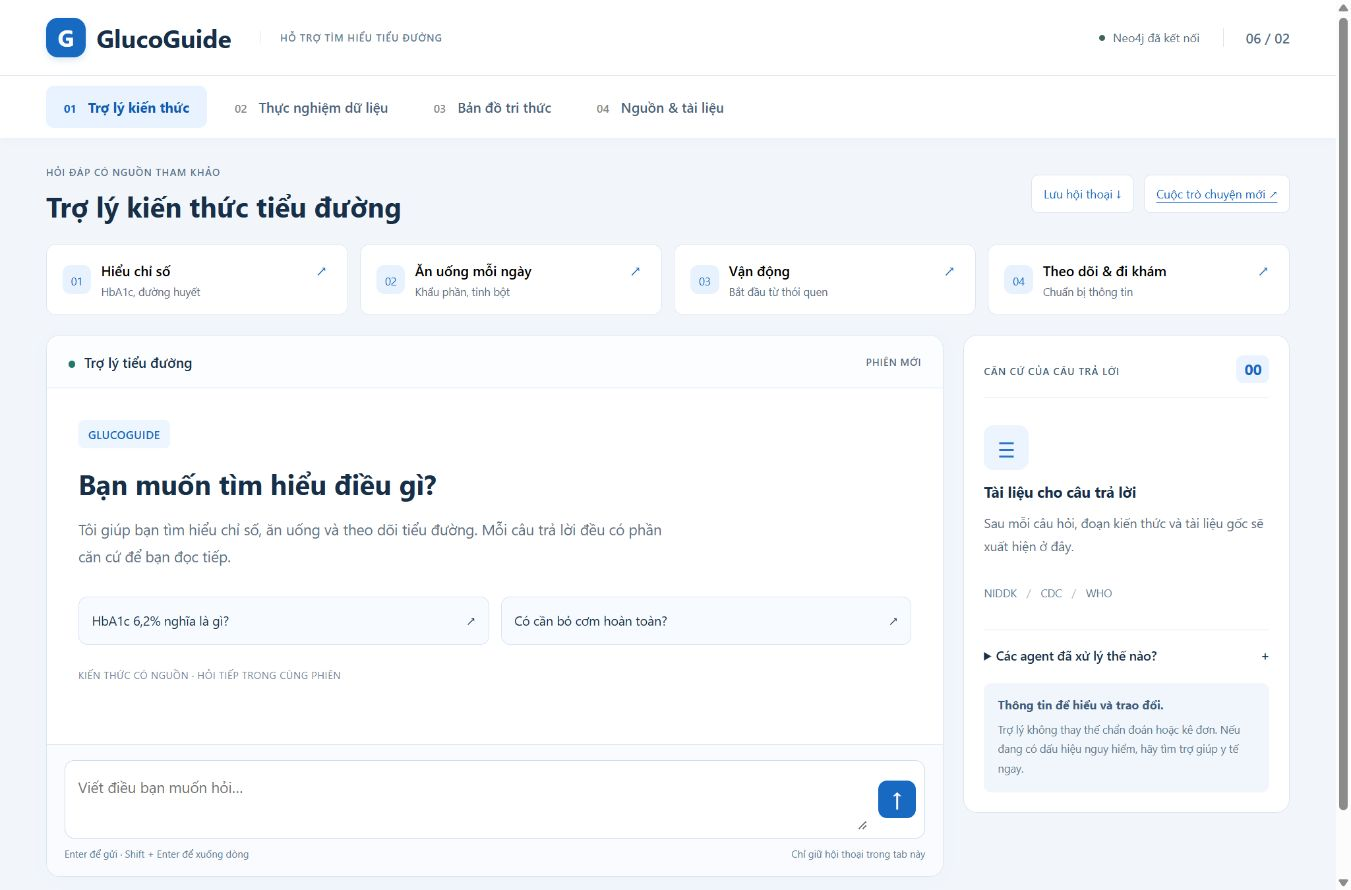
\includegraphics[width=\linewidth]{demo-home.png}\caption{Giao diện trợ lý tiểu đường với nhóm chủ đề, vùng hội thoại và tài liệu đối chiếu.}\end{figure}
\subsection{Ngữ cảnh, phạm vi và cơ chế trả lời}
API tiếp nhận history gồm tối đa 12 thông điệp, mỗi thông điệp tối đa 3.000 ký tự, role chỉ là user hoặc assistant. Khi câu hiện tại là câu hỏi tiếp nối ngắn, lớp luật tìm chủ đề có thể nhận diện trong những câu hỏi người dùng trước đó. Ví dụ, sau câu ``HbA1c là gì?'', câu ``Vậy 7,1\% thì sao?'' được hiểu là tiếp tục về HbA1c. Các con số cũ không tự điền vào câu mới; hệ thống không dựng hồ sơ lâm sàng đầy đủ từ lịch sử.

Lịch sử nằm trong bộ nhớ JavaScript của tab, không được ghi vào cơ sở dữ liệu. Nút cuộc trò chuyện mới xóa lịch sử ở giao diện. Tải lại trang cũng bắt đầu phiên mới. Nút lưu hội thoại tạo tệp văn bản cục bộ theo thao tác người dùng. Máy chủ xử lý lịch sử trong từng yêu cầu; đây chưa phải hệ thống quản lý bệnh án hoặc bộ nhớ dài hạn.

Module conversation.py phân loại chủ đề và kiểm tra đơn vị bằng luật. Nếu có chủ đề rõ, nó chọn các mã tài liệu đã định nghĩa; trường hợp còn lại dùng TF-IDF. Vì vậy phần truy xuất là kết hợp luật định tuyến và tìm kiếm văn bản. ``Hội thoại'' trong trace là nhãn của module luật, không phải một agent tự chủ mới. Bốn đối tượng agent và MessageBus vẫn là các thành phần thực thi được mô tả trong kiến trúc.

Bộ phản hồi sử dụng các đoạn văn trong KB cùng phần giải thích được định dạng theo luật. Không có LLM được gọi, nên khả năng hiểu cách diễn đạt lạ, phủ định phức tạp hoặc nhiều ý đồng thời còn hạn chế. Đây là chatbot chuyên miền có phạm vi giới hạn, không tương đương hệ tư vấn y khoa tự động.
\subsection{Kiểm tra chỉ số trước khi giải thích}
HbA1c phải có đơn vị phần trăm; nếu thiếu đơn vị, chatbot hỏi lại thay vì tự coi là phần trăm. Đường huyết nhận mg/dL hoặc mmol/L; quy đổi xấp xỉ theo hệ số 18 được công bố trong câu trả lời. Số đo sau ăn hoặc không rõ thời điểm không bị tự áp bảng lúc đói. Khi phát hiện nội dung thai kỳ hoặc trẻ em trong ngữ cảnh được xét, hệ thống không dùng bảng người lớn để diễn giải cá nhân.

Các ngưỡng và lưu ý được rà soát theo NIDDK; hướng dẫn hạ đường huyết tham chiếu CDC. Luật về dấu hiệu khẩn cấp ưu tiên lời nhắc tìm trợ giúp y tế. Câu hỏi liều thuốc được chuyển về giải thích phạm vi và thông tin chuẩn bị cho bác sĩ. Luật nhận diện bằng từ khóa vẫn có thể bỏ sót cách diễn đạt chưa kiểm thử; kết quả đạt kiểm thử không phải chứng nhận an toàn lâm sàng.
\subsection{Nối mô hình với hội thoại và so sánh đầu vào}
Sau khi suy luận, người dùng có thể bấm ``Đưa kết quả sang trò chuyện'' để xem giải thích phạm vi và căn cứ. Thao tác giữ kết quả thực từ API, không dựng một dự đoán mới trong JavaScript. Người dùng cũng có thể đổi một trường và chạy lại để xem khác biệt so với lần chạy trước. Với mẫu hồi quy đã lưu, đổi BMI từ 32,1 thành 28 cho đầu ra từ 207,53 thành 179,64, chênh lệch khoảng -27,89 điểm trong lượt demo được kiểm tra. Đây là độ nhạy của mô hình trên đầu vào giả định; không suy ra hiệu quả điều trị hay mục tiêu giảm cân.
\subsection{Tra cứu KB và sử dụng Neo4j}
Mục Nguồn \& tài liệu có tra cứu không dấu trên 21 đoạn kiến thức. Mỗi kết quả có nội dung, nguồn gốc và nút hỏi trợ lý. GET /api/knowledge trả các đoạn văn và thông tin nguồn; GET /api/status kiểm tra kết nối Neo4j và số lượng nút, cạnh.

Neo4j đã cài cục bộ trên máy thực hiện. Khi trạng thái kết nối thành công, người dùng vào Bản đồ tri thức, chọn HbA1c, bấm nút hoặc mã tài liệu để đọc căn cứ. Đồ thị có 60 khái niệm và 32 quan hệ. Tài liệu classification\_scope có văn bản nhưng chưa có bộ ba; chọn tài liệu này trả về không có cạnh thay vì hiển thị các cạnh không liên quan. Khi dịch vụ tắt, chạy start-neo4j.ps1 từ thư mục project. Muốn dùng Neo4j Browser, mở localhost:7474/browser và dùng tài khoản trong cấu hình cục bộ; không đưa mật khẩu vào báo cáo hoặc GitHub.
\subsection{Kiểm thử bổ sung và thiết bị}
Tệp scripts/test\_chatbot.py kiểm tra 16 tình huống hội thoại và 4 điều kiện API: lời chào, HbA1c, tiếp nối một và nhiều lượt, thiếu đơn vị, lúc đói, sau ăn, hạ đường huyết, khẩn cấp, câu hỏi kiến thức, liều thuốc, thai kỳ, ăn uống, ngoài miền và tách ngữ cảnh giữa yêu cầu. Bốn điều kiện API kiểm tra role không hợp lệ, lịch sử vượt giới hạn, tìm kiếm không dấu và trạng thái Neo4j. Cả 20 kiểm tra đạt; 8 kịch bản tích hợp trước đó cũng được chạy lại và đạt. Kết quả lưu tại results/chatbot\_scenarios.json và results/api\_scenarios.json.

Kiểm tra thủ công trên web bao gồm bấm nguồn sang đồ thị, chọn nút, tài liệu không có cạnh, phân loại, hồi quy, thay đổi đầu vào, chuyển kết quả sang chat, tìm kiếm không dấu và xóa phiên. Bố cục được kiểm tra tại viewport desktop 1366\,px và điện thoại 390\,px; trang chat không bị tràn ngang ở kích thước điện thoại kiểm tra. Chưa kiểm thử toàn bộ trình duyệt hay đánh giá trải nghiệm với người dùng thật.
\begin{figure}[htbp]\centering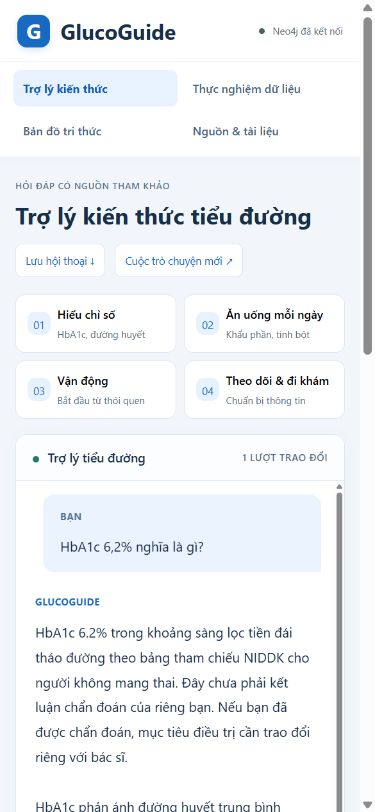
\includegraphics[height=.48\textheight,keepaspectratio]{demo-mobile.png}\caption{Bố cục điện thoại: điều hướng hai hàng và hội thoại một cột.}\end{figure}
\clearpage
